% !TEX TS-program = pdflatex
% !TEX encoding = UTF-8 Unicode

% This is a simple template for a LaTeX document using the "article" class.
% See "book", "report", "letter" for other types of document.

\documentclass[14pt]{article} % use larger type; default would be 10pt
\usepackage[14pt]{extsizes}

\usepackage[utf8]{inputenc} % set input encoding (not needed with XeLaTeX)

%%% Examples of Article customizations
% These packages are optional, depending whether you want the features they provide.
% See the LaTeX Companion or other references for full information.

%%% PAGE DIMENSIONS
\usepackage{geometry} % to change the page dimensions
\geometry{a4paper} % or letterpaper (US) or a5paper or....
\geometry{left=30mm, top=20mm, bottom=20mm, right=15mm} % for example, change the margins to 2 inches all round
% \geometry{landscape} % set up the page for landscape
%   read geometry.pdf for detailed page layout information

\usepackage{graphicx} % support the \includegraphics command and options
\usepackage{epstopdf}

\usepackage{amsmath}

%\usepackage[parfill]{parskip} % Activate to begin paragraphs with an empty line rather than an indent

%%% PACKAGES
\usepackage{booktabs} % for much better looking tables
\usepackage{array} % for better arrays (eg matrices) in maths
\usepackage{paralist} % very flexible & customisable lists (eg. enumerate/itemize, etc.)
\usepackage{verbatim} % adds environment for commenting out blocks of text & for better verbatim
\usepackage{subfig} % make it possible to include more than one captioned figure/table in a single float
\usepackage[english, russian]{babel}
\usepackage[hidelinks]{hyperref}
\usepackage{bookmark}
% These packages are all incorporated in the memoir class to one degree or another...
%\usepackage{tempora}

%%% HEADERS & FOOTERS
\usepackage{fancyhdr} % This should be set AFTER setting up the page geometry
\pagestyle{fancy} % options: empty , plain , fancy
\renewcommand{\headrulewidth}{0pt} % customise the layout...
\lhead{}\chead{}\rhead{}
\lfoot{}\cfoot{\thepage}\rfoot{}

%%% SECTION TITLE APPEARANCE
%\usepackage{sectsty}
%\allsectionsfont{\sffamily\mdseries\upshape} % (See the fntguide.pdf for font help)
% (This matches ConTeXt defaults)

%%% ToC (table of contents) APPEARANCE
\usepackage[nottoc,notlof,notlot]{tocbibind} % Put the bibliography in the ToC
\usepackage[titles,subfigure]{tocloft} % Alter the style of the Table of Contents
\renewcommand{\cftsecfont}{\rmfamily\mdseries\upshape}
\renewcommand{\cftsecpagefont}{\rmfamily\mdseries\upshape} % No bold!
\linespread{1.5}

\usepackage{indentfirst}

%%% END Article customizations

%%% The "real" document content comes below...

\title{Brief Article}
\author{The Author}
%\date{} % Activate to display a given date or no date (if empty),
         % otherwise the current date is printed 

\sloppy\begin{document}
\begin{titlepage}

\begin{center}
{\small \bf Санкт-Петербургский государственный университет

Кафедра астрономии}
\end{center}

\vspace{2cm}
%\maketitle
\begin{center}
  \large{\bf Кинематический анализ звезд каталога TGAS}
 \end{center}

\vspace{3cm}

\hspace{8cm}\parbox{8cm}{	% Лучше делать так, чем с помощью flushright - сдвинутый текст будет выровнен по левому краю.

\footnotesize{{\bf Выпускная квалификационная работа}\\
студента группы 13.С04-мм\\
П. В.\,Мовсесяна}  % Собственное отчество тоже надо бы указывать. :) 

\vspace{1cm}

{\bf Научный руководитель}\\
А. С.\,Цветков \\  % Есть такое правило - если нет никаких конкретных причин так не делать, то инициалы указываются перед фамилией, а не после. Исключения - тексты вроде милицейского протокола или списки с сортировкой по фамилиям в алфавитном порядке
}


\vfill % Лучше так - то, что ниже, окажется сдвинутым настолько низко, насколько возможно.

\begin{center}
\small {Санкт-Петербург

2018}
\end{center}

\end{titlepage}

\tableofcontents
\newpage

\section{Введение}

Первый раз идея астрометрического спутника была реализована в проекте Hipparcos, запущенном в 1989 году. В октябре 2000 года были начаты работы по реализации проекта. В 2013 году аппарат был запущен с космодрома Куру, а 8 января 2014 достиг своей орбиты вблизи точки $L_2$.

Аппарат был запущен 19 декабря 2013 года в 9:12 UTC, достиг орбиты через несколько недель. Планируется, что он проведет на орбите минимум 5 лет. Использовалась ракета-носитель <<Союз>> с разгонным блоком <<Фрегат>>. Масса аппарата составляет 2030 кг, из которых 710 кг полезной нагрузки, 920 кг -- сервисный модуль и 400 кг ракетного топлива.

Gaia двигается по орбите Лиссажу с периодом 180 суток. Размеры орбиты составляют $3.4\cdot10^5 \times 9\cdot10^4$ км. Орбита рассчитана так, чтобы аппарат не попадал в тень Земли.

Аппарат вращается со скоростью $1^\circ$ в минуту, угол между полями зрения (базовый угол BAM) составляет $106.5^\circ$. Ось вращения находится под углом $45^\circ$ к направлению на Солнце, период прецессии равен 63.12 суткам.

Аппарат выполняет три основные функции. В его ранних версиях эти функции выполнялись тремя инструментами. Сейчас они встроены в один инструмент, используя общую оптику. Астрометрический инструмент (ASTRO) занимается измерениями угловых положений объектов, получает 5 параметров: положение (2 угла), собственное движение (2 производных положения) и параллакс. Фотометрический инструмент получает непрерывные спектры в диапазоне длин волн 320--1000 нм и обеспечивает цветовую калибровку ASTRO. Спектрометр лучевых скоростей (RVS) предоставляет лучевые скорости и спектральные данные высокого разрешения в узком диапазоне 847--874 нм.

Дизайн аппарата характеризуется двойным телескопом с общей структурой и общей фокальной плоскостью. Оба телескопа используют трехзеркальную анастигматическую схему. Лучи объединяются, затем перенаправляются в фокальную область. В качестве основного материала используется SiC, что позволяет достичь малой массы и стабильности в космосе. Благодаря этому используется пассивный контроль температуры. Главные зеркала имеют размеры $1.45\times0.5$ м и фокусное расстояние 35 м.

ASTRO имеет 62 ПЗС в фокальной плоскости, где два поля зрения собраны в астрометрическое поле (AF). ПЗС работают в сканирующем режиме.\\\\
\begin{tabular}{|c|c|c|}
\hline
\multicolumn{3}{|c|}{Ошибка параллакса}\\
\hline
Спектральный класс & Видимая звездная величина & $\sigma(\pi)$, $\mu as$\\
\hline
\raisebox{-4ex}[0cm][0cm]{B2V} &<10 &<7\\
\cline{2-3}
& 15 & <25\\
\cline{2-3}
& 20 & <300\\
\hline
\raisebox{-4ex}[0cm][0cm]{G2V} &<10 &<7\\
\cline{2-3}
& 15 & <24\\
\cline{2-3}
&20 & <300\\
\hline
\raisebox{-4ex}[0cm][0cm]{M6V} &<10 &<7\\
\cline{2-3}
& 15 & <12\\
\cline{2-3}
&20 & <100\\
\hline
\end{tabular}\\

Фотометр будет измерять распределение энергии в спектрах объектов, что позволит получить такие параметры, как светимость, эффективную температуру, массу, возраст. Его работа осуществляется при помощи дисперсионной оптики для коротких волн (BP 320--660 нм) и длинных волн (RP 650--1000 нм). Призмы расположены максимально близко к фокальной плоскости. Для фотометра выделены две полосы ПЗС. Длина получаемых спектров составляет 30 пикселей для BP и RP. Предполагается ошибка определения звездной величины в диапазоне $10\mbox{--}200\times10^{-3\mbox{ }m}$.

RVS будет получать лучевые скорости при помощи наблюдений в ближнем ИК (847--874 нм) с разрешением 11500 ($\lambda/\Delta\lambda$). Для этого используется массив ПЗС $3\times4$.

В фокальной плоскости находятся 106 ПЗС, произведенных компанией E2V. Разрешение каждой составляет $4500\times1966$ пикселей при линейных размерах $4.726\times6.0$ см. Объект проходит по матрице за 4.42 секунды. Рабочая температура равна -115 $^\circ$С.
\\\\
\begin{tabular}{|p{3.5cm}|p{2.5cm}|p{8cm}|}
\hline
Назначение&Количество ПЗС&Подробности\\
\hline
Ориентация &4 & 2 сенсора фронта волны, 2 матрицы для мониторинга BAM\\
\hline
Распознавание объектов &14&$2\times7$ по 7 на телескоп\\
\hline
Астрометрия (AF) & 62 & $8\times7$, $1\time6$\\
\hline
Фотометрия (BP, RP) & 14 & 7 синих, 7 красных\\
\hline
Спектрометрия (RVS) & 12& $3\times4$\\
\hline
\end{tabular}\\

14 сентября 2016 был опубликован Gaia Data Release 1, состоящий из двух каталогов: Gaia и Tgas. Далее речь идти будет о Tgas. Tgas (Tycho-Gaia Astrometric Solution) -- каталог отождествленных с Hipparcos и Tycho-2 объектов, содержащий данные о пяти астрометрических параметрах. Data Release 2 был опубликован 25 апреля 2018. Релиз финального каталога планируется в 2022 году.
%\newpage\section{TGAS: общие сведения}
%Была написана программа, обеспечивающая корректное чтение файлов каталога и инициализацию пустых полей. С ее помощью был проведен анализ полученных параллаксов и построена зависимость относительной ошибки расстояния от расстояния.
%\begin{figure}[h!]
%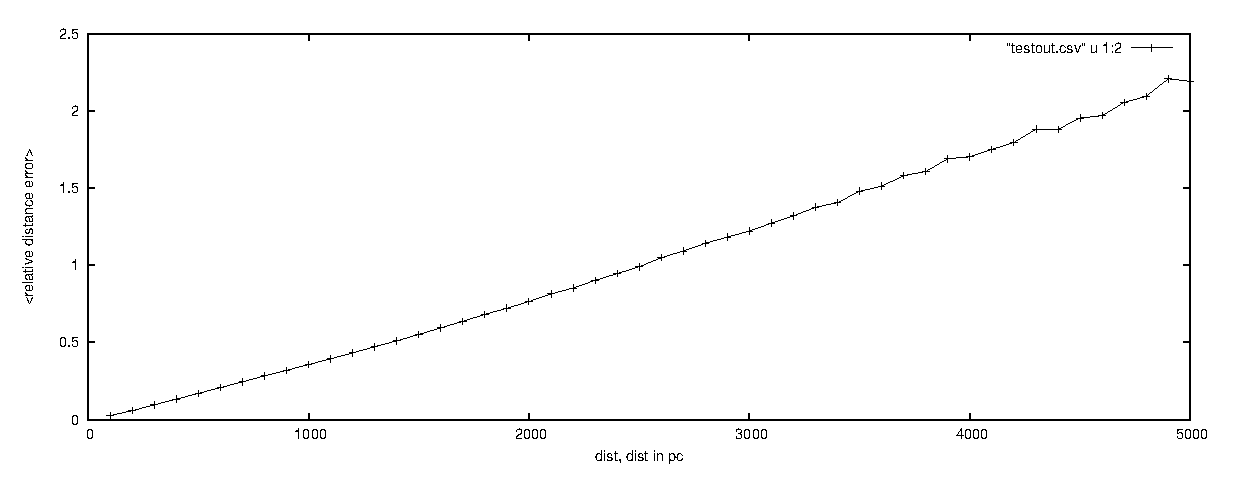
\includegraphics[width=1\linewidth]{distvserr.eps}
%\end{figure}

%У Hipparcos относительная погрешность на расстоянии 2 кпк составляла 2.83, когда на графике выше она 0.765.

%Также был построен график количества объектов от расстояния.
%\begin{figure}[h!]
%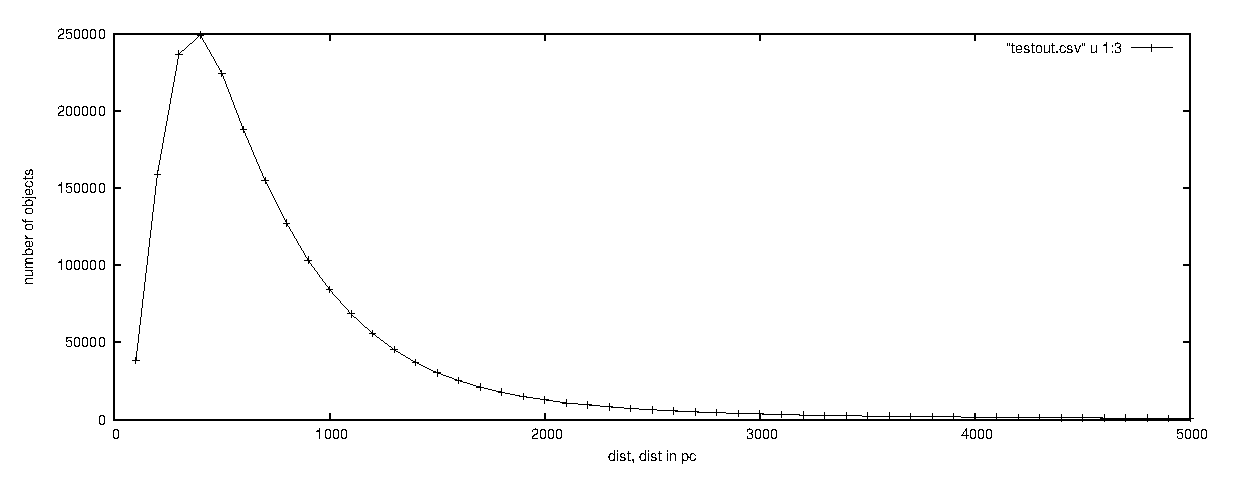
\includegraphics[width=1\linewidth]{distvsN.eps}
%\end{figure}\newpage

%Была построена карта объектов. Использовалась проекция Хаммера.
%\begin{figure}[h!]
%\includegraphics[width=1\linewidth]{galsph.jpg}
%\end{figure}

%Далее работа проводилась не с каждым объектом, а с усредненными характеристиками по HEALPIX-площадкам.

%Была построена карта плотности объектов (в тысячах).
%\begin{figure}[h!]
%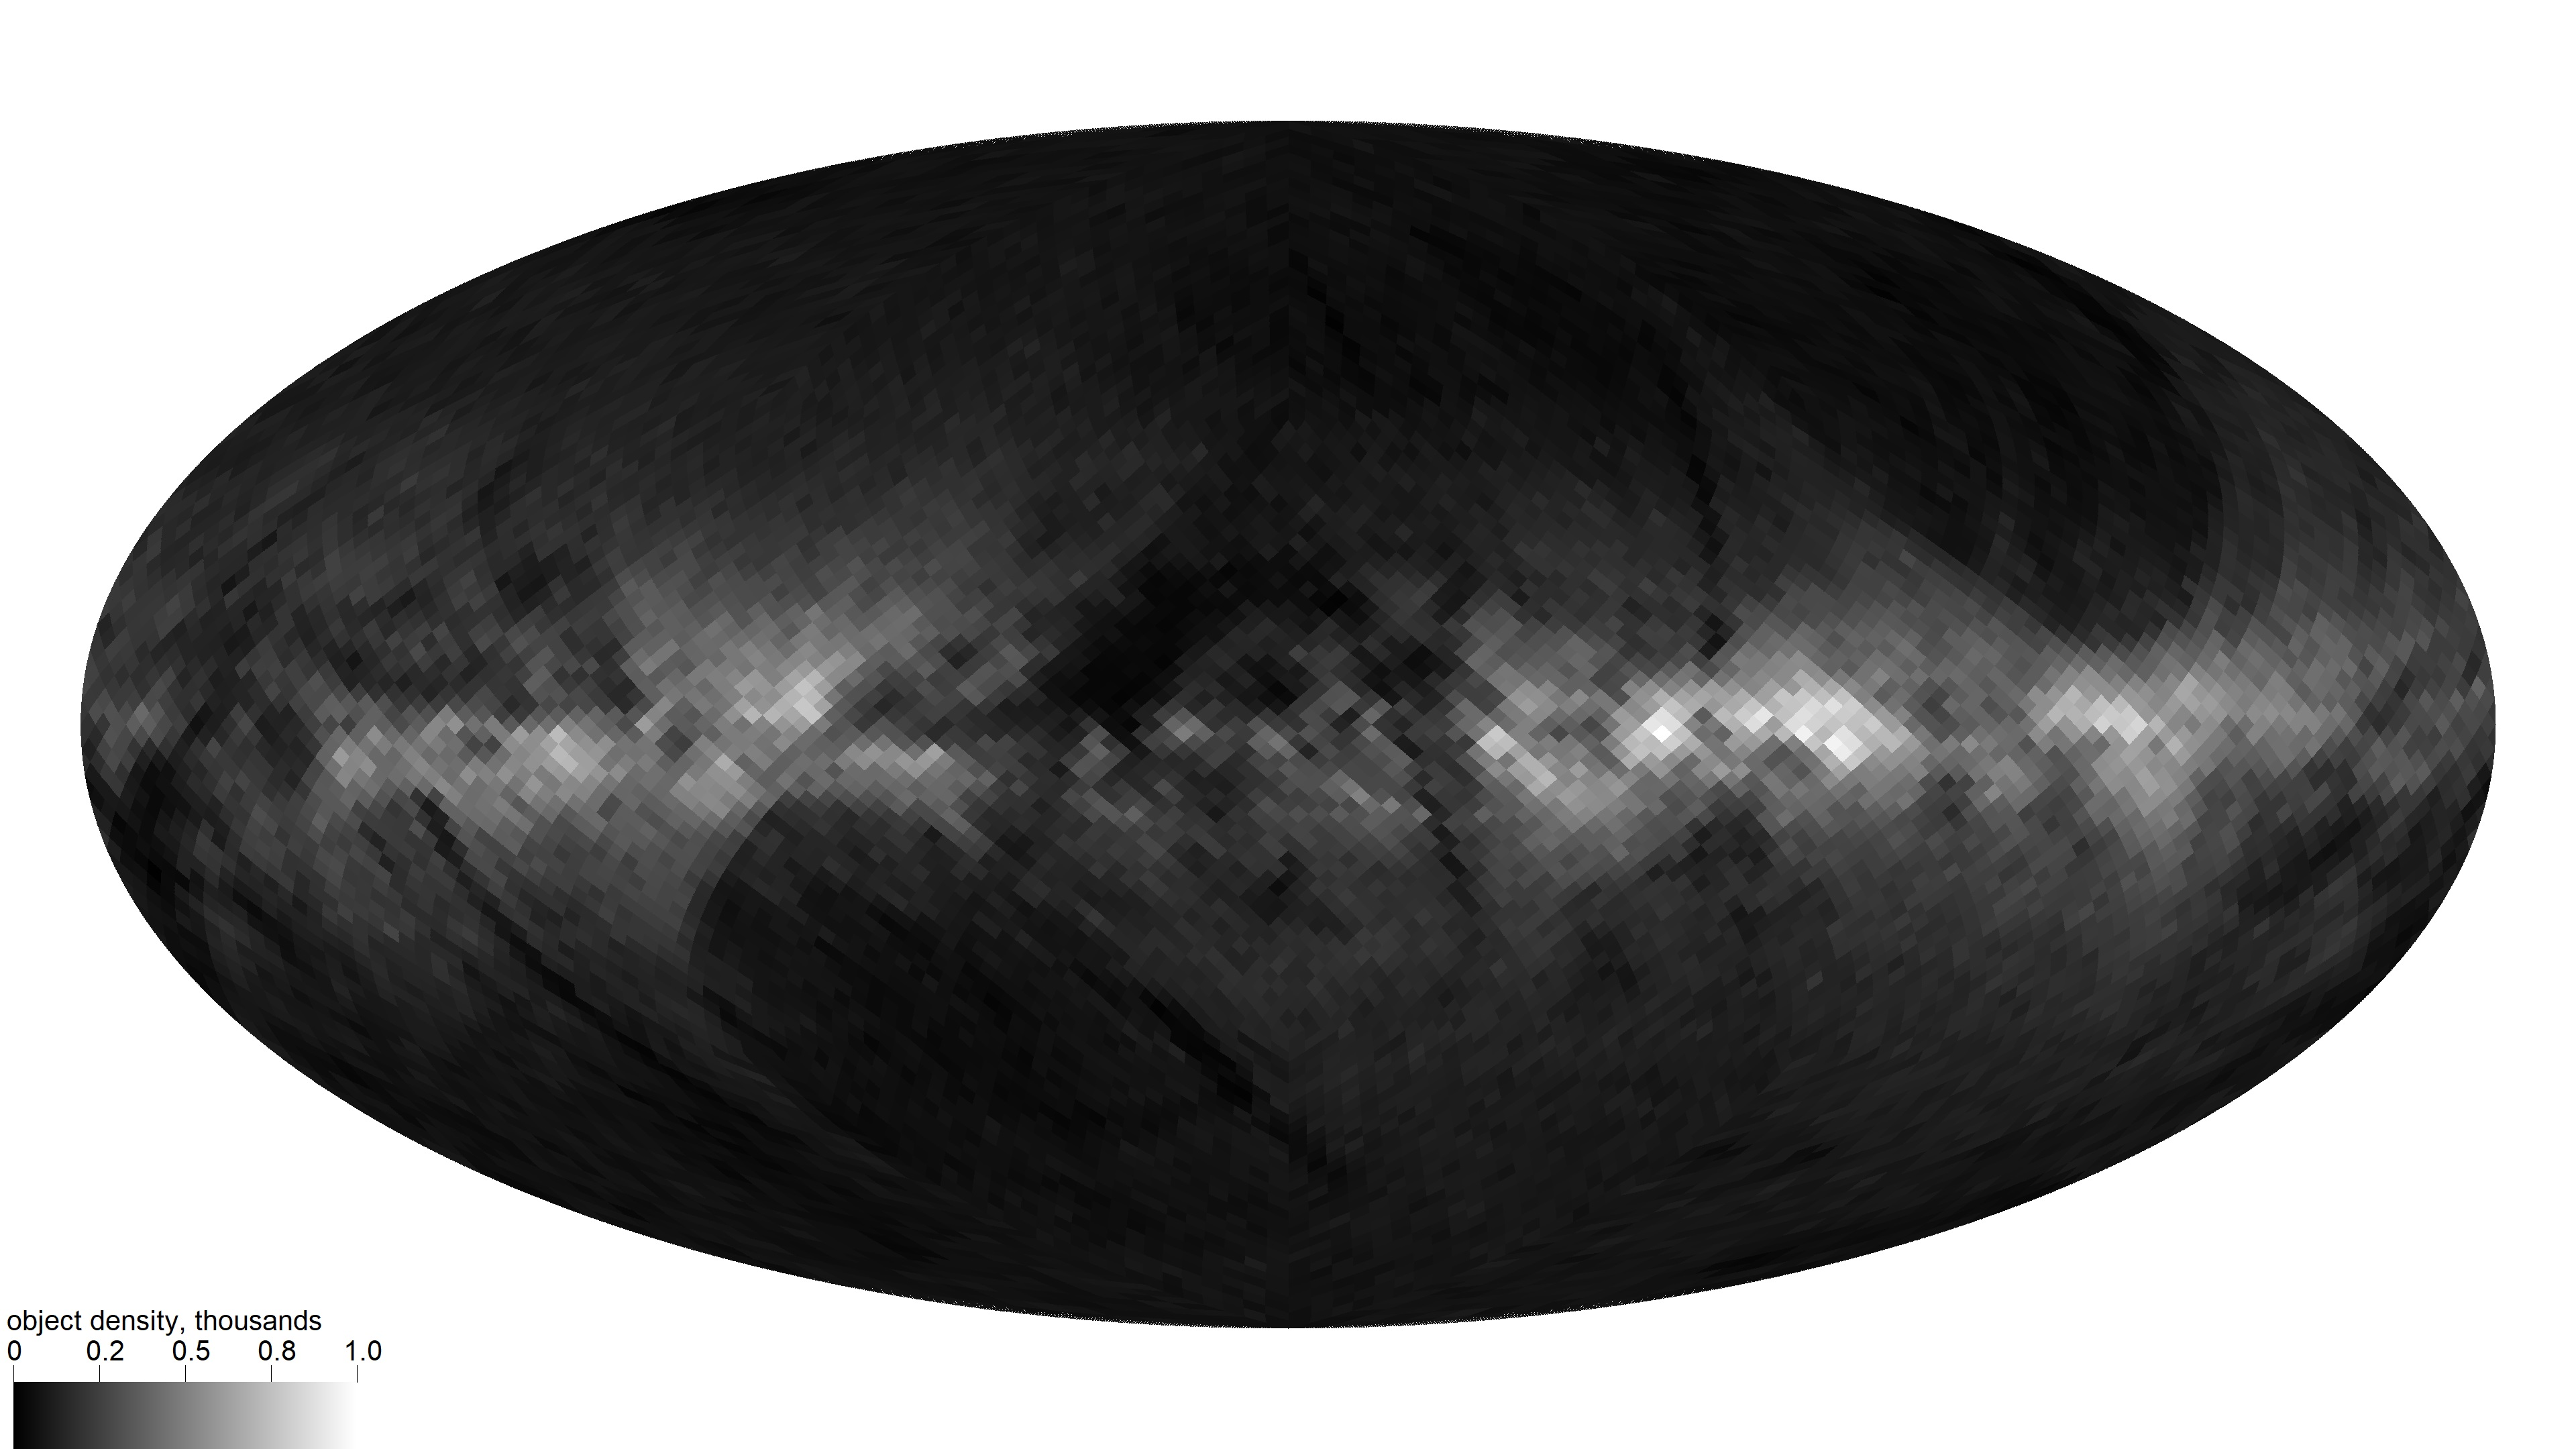
\includegraphics[width=1\linewidth]{healpdens.jpg}
%\end{figure}\newpage

%После этого я построил карту средних расстояний до объектов.
%\begin{figure}[h!]
%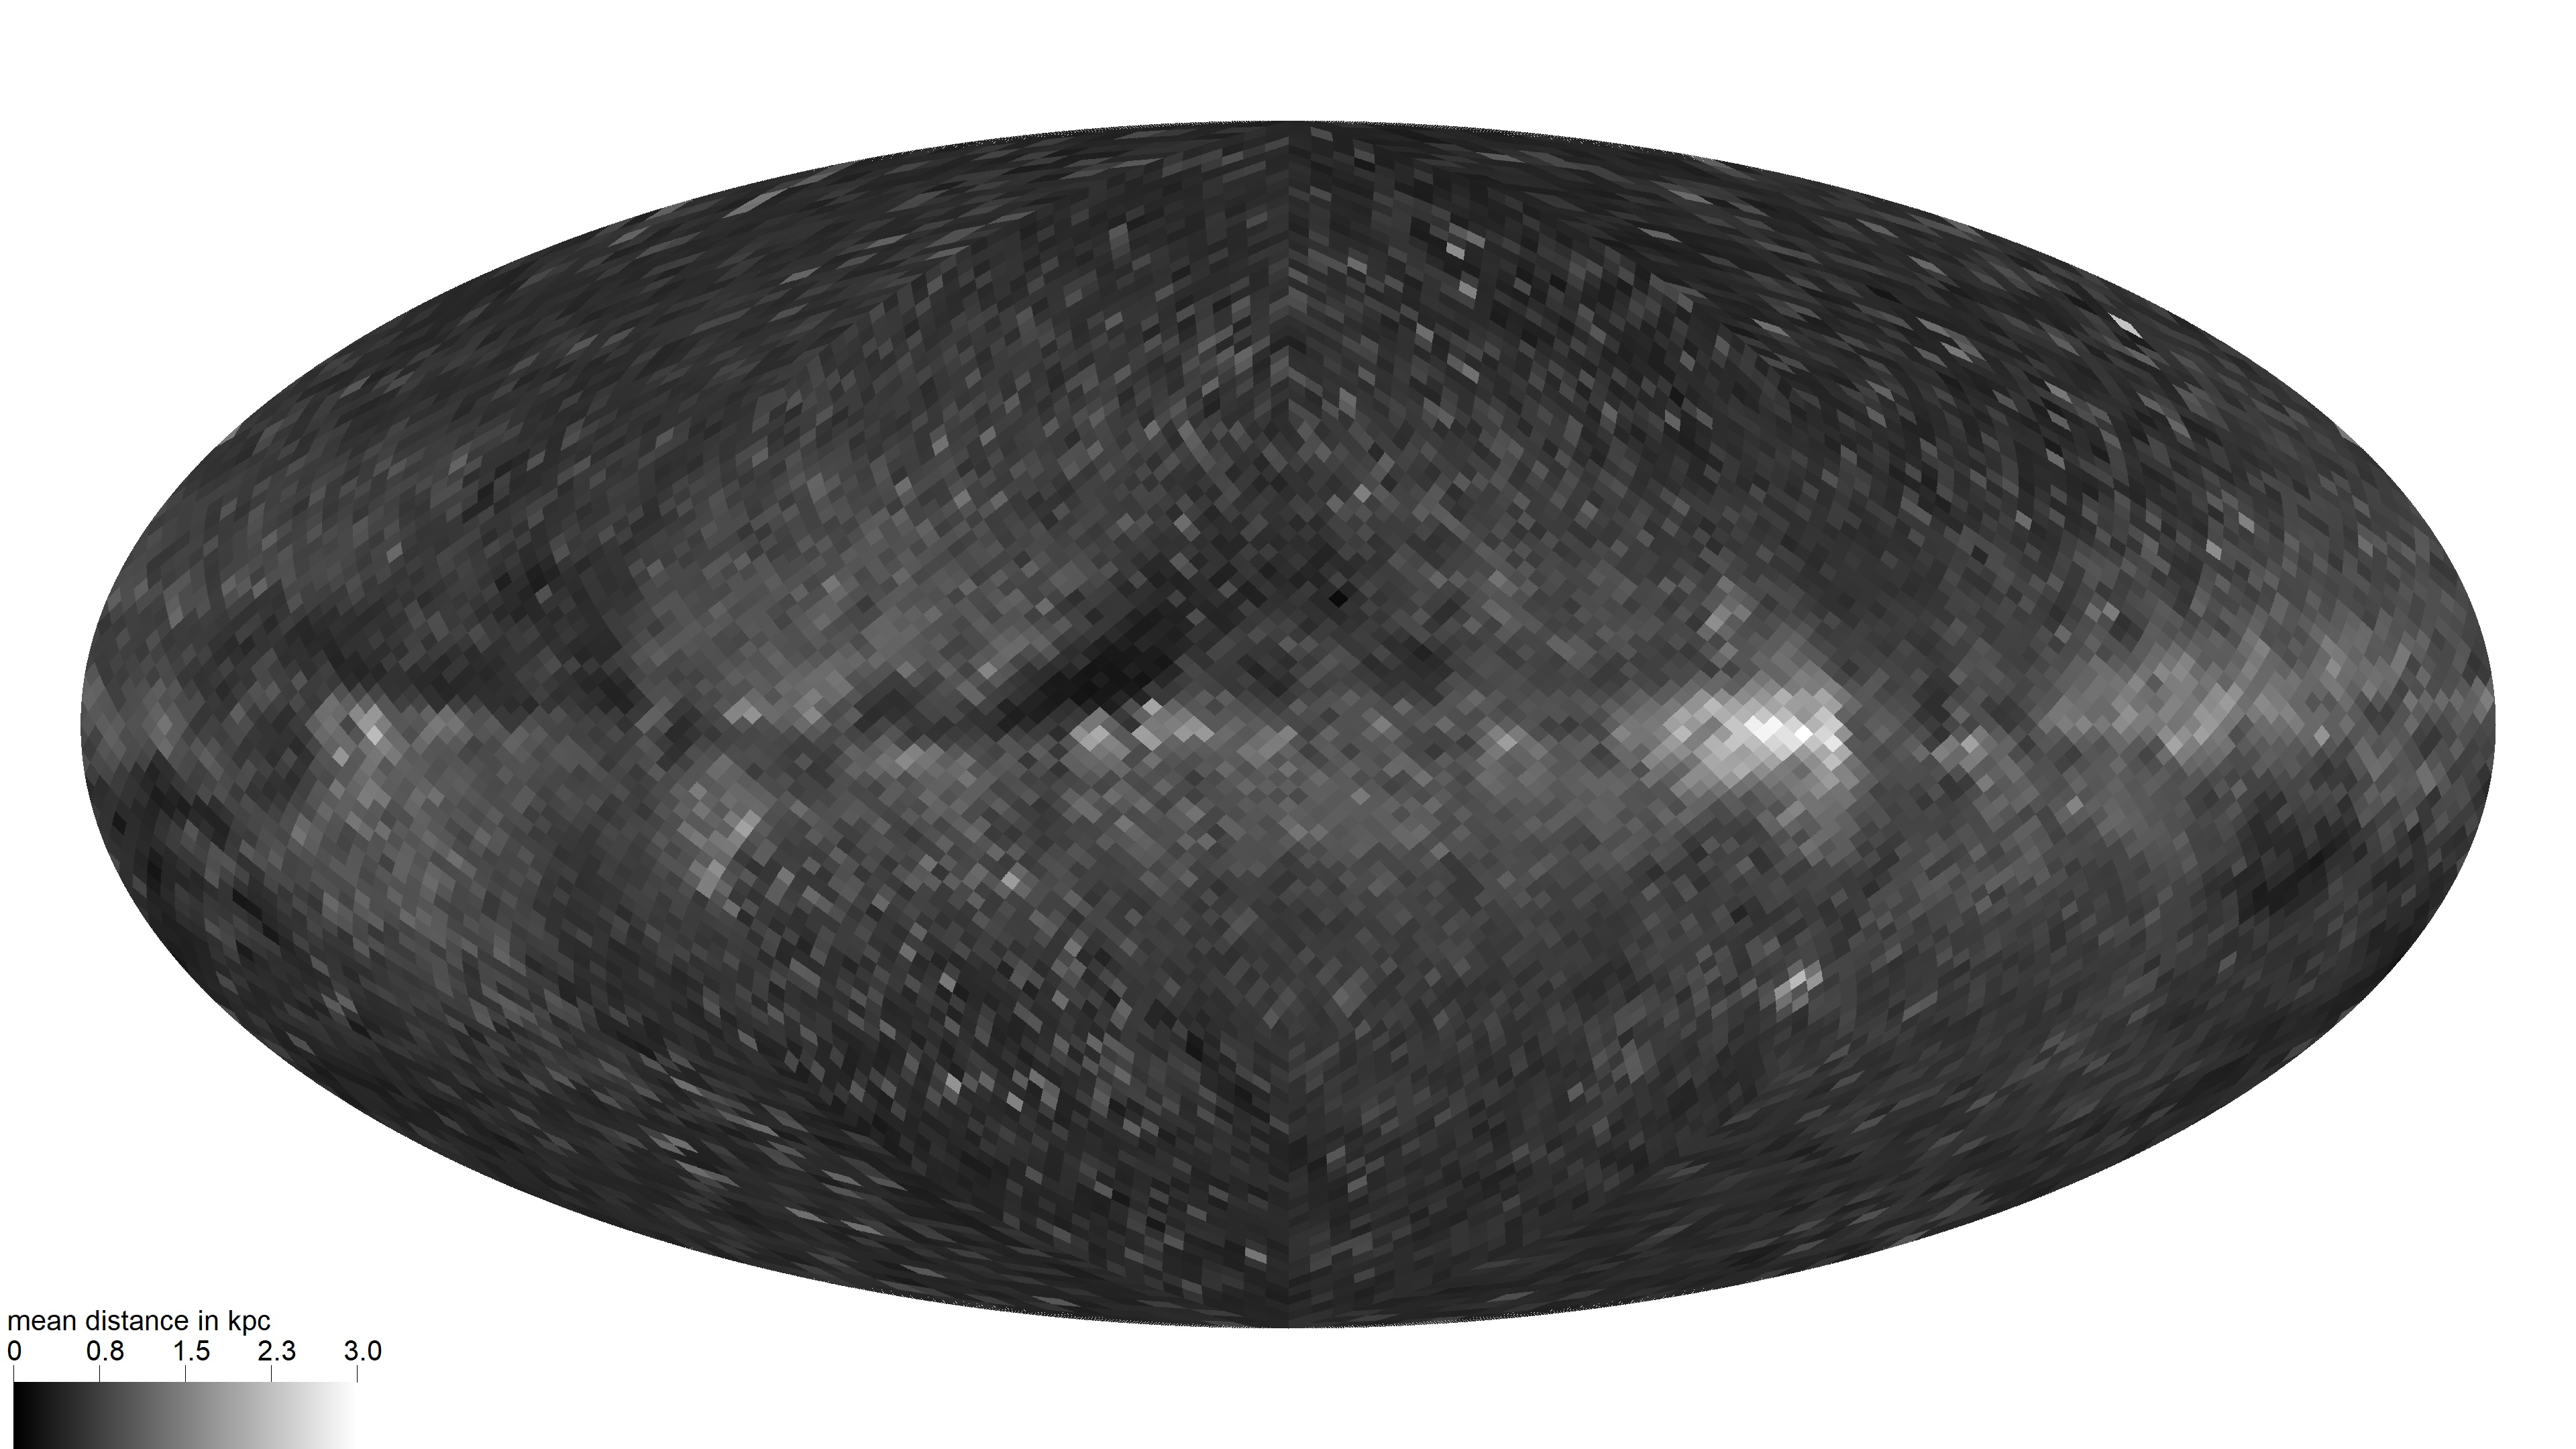
\includegraphics[width=1\linewidth]{healpdistmap.jpg}
%\end{figure}

\section{Пикселизация данных на сфере}

\subsection{HEALPix}
HEALPix -- акроним \textbf{H}ierarchical \textbf{E}qual \textbf{A}rea iso\textbf{L}atitude \textbf{Pix}elization (Иерархическая равноплощадная изоширотная пикселизация).

Разрешение карты описывается параметром $N_{side}$, показывающим число разбиений базовых ячеек. Центры всех ячеек одного кольца расположены на одинаковой широте и равноудалены друг от друга по долготе. Кольца делятся на полярные ($\left|\cos\theta\right|>\frac{2}{3}$) и экваториальные ($\left|\cos\theta\right|<\frac{2}{3}$). В экваториальных кольцах ячеек составляет $N_{eq}=4N_{side}$, остальные принадлежат полярным кольцам. Всего $4N_{side}-1$ колец.
HEALPix карта имеет $N_{pix}=12N_{side}^2$ ячеек одинаковой площади $\Omega_{pix}=\frac{\pi}{3N_{side}^2}$.
%\subsubsection{Положения ячеек}
Положения на сфере определяются с помощью $z \equiv \cos\theta$ и $\phi$, где $\theta \in \left[0,\pi\right]$ -- полярное расстояние, измеряемое от северного полюса, а $\phi \in\left[0,2\pi\right]$ -- долгота в радианах, отсчитывающаяся на восток.

Положения центров ячеек вычисляются следующим образом:

$p$ -- номер площадки\\
Для северной полярной шапки:\\
$p_h=\frac{p+1}{2}$\\
$1\le i<N_{side}$ -- индекс кольца\\
$1\le j<4i$ -- индекс ячейки внутри кольца\\
$$i=\left\lfloor\sqrt{p_h-\sqrt{\left\lfloor p_h\right\rfloor}}\right\rfloor+1$$
$$j=p+1-2i\left(i-1\right)$$
$$z=1-\frac{i^2}{3N_{side}^2}$$
$$\phi=\frac{\pi}{2i}\left(j-0.5\right)$$\\
Для северного экваториального пояса:\\
$p'=p-2N_{side}\left(N_{side}-1\right)$\\
$N_{side}\le i\le 2N_{side}$\\
$1\le j\le 4N_{side}$
$$i=\left\lfloor\frac{p'}{4N_{side}}\right\rfloor + N_{side}$$
$$j=(p' \mod 4N_{side}) +1$$
$$z=\frac{4}{3}-\frac{2i}{3N_{side}}$$
$$\phi=\frac{\pi}{2N_{side}}\left(j-\frac{\left(i-N_{side}+1\right)\mod 2}{2}\right)$$
Для южного полушария положения центров получаются симметрично относительно экватора ($z=0$) 
%\section{Заключение}
%В ходе работы было разработано программное обеспечение для чтения и обработки каталога Tgas. Были получены графики зависимостей относительной ошибки определения расстояния от расстояния до объекта и количества объектов от расстояния. Также были построены карты объектов, распределения их по небесной сфере и распределения средних расстояний по сфере.
\newpage
\begin{thebibliography}{99}
\bibitem{gaiasite}ESA Science \& Technology: Gaia \url{http://sci.esa.int/gaia/}
\bibitem{healp1}K.\,M.\,Gorski, E.\,Hivon, A.\,J.\,Banday, B.\,D.\,Wandelt, F.\,K.\,Hansen, M.\,Reinecke, M.\,Bartelman: HEALPix -- a Framework for High Resolution Discretization, and Fast Analysis of Data Distributed on the Sphere \url{https://arxiv.org/abs/astro-ph/0409513}

\end{thebibliography}

\end{document}
